 % -*- encoding: UTF8 -*-
%
%%*****************************************************************************
%%				Fabrication and Assembly										                                        
%%*****************************************************************************
\chapter{Fabrication and Assembly}
\label{Ch:Fab}	

\begin{figure}[h!]\centering 
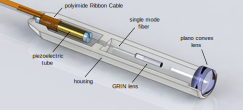
\includegraphics[width=\columnwidth]{figures/40_Fabrication/overview.pdf}
      \caption{CAD of the single modality demonstrator with the top of the housing removed. Total length: \SI{9}{\milli\meter}.}
      \label{fig:overview}
\end{figure}

The probe shown in Figure \ref{fig:overview} was built as a demonstrator of the fiber scanner design and evaluation of the optical performance of the OCT beam path.

The piezoelectric actuator with four outer gold electrodes to control the lateral movement of the scanner is supplied by PI Ceramic. The addressing of these electrodes is realized by a polyimide-based ribbon cable, which is wrapped around the piezoelectric tube. Conductive glue is applied through via holes in the ribbon cable to enable the connection between the platinum from the conductors and the gold pads of the piezotube surface. The single mode fiber is centered in the piezoelectric tube using small FR-2 discs and the GRIN lens bonded to the tip of this fiber using optical adhesive. 

This arrangement enables a compact fiber scanner with a total length of \SI{9}{\milli\meter} and a resonance frequency of \SI{750}{\hertz} optimized for an OCT system with an A-Scan repetition rate of \SI{100}{\kilo\hertz}.

The following paragraphs describe the manufacturing process of the most relevant components of the probe.

%%*****************************************************************************
\clearpage
\section{Polyimide Electrodes}
%%*****************************************************************************
Due to the small diameter of the piezoactuator, contacting its electrodes reliably is not trivial. Other piezoscanner implementations use soft soldering and insulated copper wires \cite{Lee2010}, \cite{Meinert}, \cite{Huo2010}. The soldering process can damage the actuator, as it is exposed to temperatures above its Curie temperature. This methosd also increases significantly the diameter of the actuator, as a solder blob is needed. Furthermore, it requires welding by hand in a \SI{600}{\micro\meter} curved electrode -- certainly not production-friendly.



Instead, we developed a polyimide ribbon cable which is wrapped around the piezotube and addresses its 4 external electrodes with vias. Its geometry, cross section and rolled state are depicted in Figure \ref{fig:piRolled}. 

\begin{figure}[h!]\centering \includegraphics[width=10cm]{figures/40_Fabrication/PI/tubeFoil.pdf}
      \caption{\textbf{a)} Left: Photo of the polyimide ribbon cable with four vias to contact the four gold electrodes of the piezoelectric tube. Right: Piezotube.
      \textbf{b)} Schematic of one via and its cross section. The platinum around the via is partly uncovered to improve the electrical connection between the cable and the piezoelctric tube.
      \textbf{c)} Photo of a polyimide ribbon cable, wrapped around the piezoelectric tube that is electrical connected through the vias by conductive glue.}
      \label{fig:piRolled}
\end{figure}

It is manufactured using a cleanroom process similar to the one used for cuff electrodes for nerve stimulation \cite{Rodriguez2000} and consists of platinum tracks and via holes embedded in a polyimide substrate. One end the cable is shaped to fit a zero insertion force (ZIF) connector. The other end can be rolled around the piezotube, allowing the bonding to its gold electrodes using conductive glue (Araldite 2020 with 80\% wt. silver particles).


\subsection{Cleanroom processing}
The polyimide ribbon cables are manufactured and singulated at wafer level. The process involves spincoating a \SI{5}{\micro\meter} layer of polyimide, over which \SI{100}{\nano\meter} of platinum is sputtered and then patterned by liftoff, defining the conductive traces. Finally, the vias, openings and external shape are patterned through reactive ion etching (RIE). This process is described in Figure \ref{fig:piProcess}.


\begin{figure}[h!]\centering 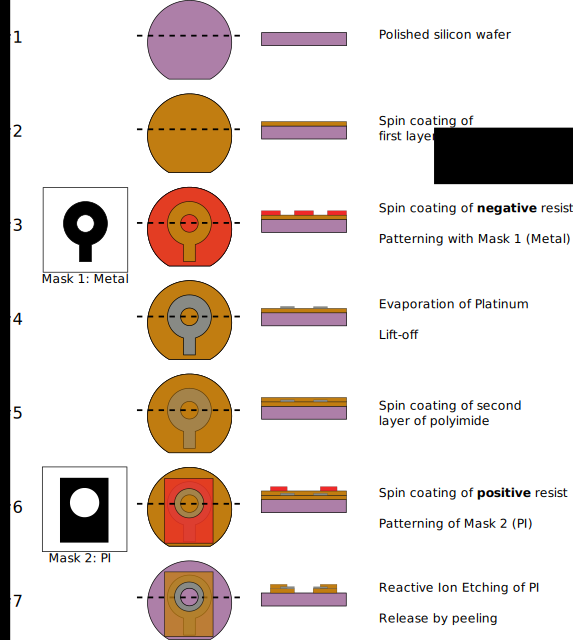
\includegraphics[width=12cm]{figures/40_Fabrication/PI/processV.pdf}
      \caption{Cleanroom fabrication process of the polyimide electrodes.}
      \label{fig:piProcess}
\end{figure}

%%*****************************************************************************
\clearpage
\section{Fiber-GRIN Bonding}
%%*****************************************************************************
\begin{figure}[h!]\centering \includegraphics{figures/40_Fabrication/FiberGRIN/fiberGRINglue.pdf}
      \caption{Fiber and GRIN lens in silicon alignment tool before (a) and after (b) bonding with UV-curable adhesive.}
      \label{fig:fiberGRINglue}
\end{figure}

The GRIN lens and the end of the fiber have to be bonded together mechanically and optically for the proper functioning of the probe. This interface is critical: first, because it is subjected to very high forces due to the oscillation of the scanner, and second, because any angular or displacement error would degrade the optical quality.

To overcome these challenges, we align the fiber to the GRIN lens using a custom made, KOH-etched silicon alignment tool. The precise geometry of the KOH-etched grooves allow a very good angle and position control of the cylindrical fiber and GRIN lens. Once in place, we apply a drop of optical UV-curable glue (NOA 76), which thanks to its wetting behavior and surface tension, creates a symmetrical wedge which provides extra mechanical integrity.

\begin{figure}[h!]\centering \includegraphics[width=10cm,draft]{figures/foo.png}
      \caption{Cross section with dimensions}
      %\label{}
\end{figure}


%%*****************************************************************************
\clearpage
\section{3D Printed Housing}
%%*****************************************************************************
\begin{figure}[h!]\centering \includegraphics[width=\columnwidth]{figures/40_Fabrication/Housing/housing.pdf}
      \caption{CAD (a) and photography (b) of the single modality probe with alignment features.}
      \label{fig:housing}
\end{figure}

%In order to assess the OCT imaging of the bimodal microendoscope, a single mode demonstrator was designed and built.

Although the bimodal probe is designed to be assembled using the silicon bench technology, we assembled the demonstrator in a 3D printed plastic housing, with no degradation in its optical quality. This is possible because the most critical alignment -- fiber to GRIN -- is performed beforehand. The rest of the components allow relatively high placement tolerances, as the beam is collimated in the region between GRIN lens and objective lens. This way, simple alignment structures which are 3D-printed in the housing allow the proper placement of all the components. 

(Material, printer, process?)

For example, in order to center the piezotube in the housing, first the fiber is retracted so that the GRIN lens seats in the GRIN alignment structure (Figure \ref{fig:grinAlignment} left). This way the piezotube is aligned in the housing and, after being glued in place, it is possible to push the fiber so that the GRIN is at its proper distance (Figure \ref{fig:grinAlignment} right). 

\begin{figure}[h!]\centering 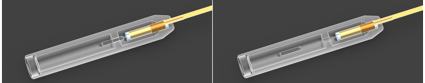
\includegraphics[width=\columnwidth]{figures/40_Fabrication/Housing/grinAlignment.pdf}
      \caption{Alignment of the piezotube-fiber-GRIN assembly in the housing.}
      \label{fig:grinAlignment}
\end{figure}

%%*****************************************************************************
\clearpage
\section{Assembly}
%%*****************************************************************************
\begin{figure}[h!]\centering \includegraphics{figures/40_Fabrication/Assy/exploded.pdf}
      \caption{Exploded view of the components of the single modality probe.}
      \label{fig:exploded}
\end{figure}
The assembly process is summarized as follows:

\begin{enumerate}
\item The GRIN lens is bonded to the end of the fiber.
\item The GRIN-fiber assembly is slid through the piezotube and centered with FR-2 fittings, which are glued to the piezotube using cyanocrilate.
\item The piezotube-fiber-GRIN assembly is placed in the housing and glued in place using cyanocrilate with help of the alignment structures.
\item The planoconvex lens is placed in the bottom half of the housing and glued using UV-curable optical glue.
\item The probe is closed with the top half of the housing and sealed with UV-curable glue.
\end{enumerate}

